\documentclass[a4paper, 12pt]{article}
\usepackage[russian]{babel}
\usepackage[T2A]{fontenc}
\usepackage[utf8]{inputenc}


\usepackage{xcolor}

\usepackage{hyperref}
\definecolor{linkcolor}{HTML}{44D663} % цвет ссылок
\definecolor{urlcolor}{HTML}{031A9B} % цвет гиперссылок

\hypersetup{pdfstartview=FitH,  linkcolor=black,urlcolor=urlcolor, colorlinks=true}

\usepackage{graphicx}

\usepackage{multirow}
\usepackage{multicol}

\usepackage{amsmath} 
\usepackage{listings}
\usepackage{xcolor}
\usepackage{color}
\usepackage{amsmath}

\definecolor{dkgreen}{rgb}{0,0.6,0}
\definecolor{gray}{rgb}{0.5,0.5,0.5}
\definecolor{mauve}{rgb}{0.58,0,0.82}
\lstset { %
	language=C++,
	backgroundcolor=\color{black!5}, % set backgroundcolor
	basicstyle=\footnotesize,% basic font setting
	tabsize=3,
	breaklines=true,
	breakatwhitespace=true,
	numbers=left,
	% Стиль литералов
}

\usepackage{pgfplots}
\pgfplotsset{compat=1.9}



\usepackage{amsmath}

\usepackage{amsmath, amsfonts}



\begin{document}
		\newpage
	
	\begin{figure}[h] % [h] означает, что рисунок будет размещен здесь, а не автоматически в конце раздела или страницы
		\centering % Выравнивание по центру
		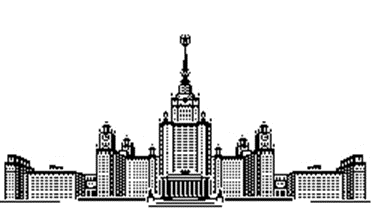
\includegraphics[width=0.5\textwidth]{МГУ.PNG} % Вставка изображения. Укажите путь к вашему изображению вместо example-image
		 % Подпись к рисунку
	
	\end{figure}
	
	\begin{center}
		\text{\large{Московский государственный университет имени М.В.Ломоносова}} \\
		
		\text{\large{Факультет вычислительной математики и кибернетики}} \\
		
		\text{\large{Кафедра математической физики}} 
	
		
	\end{center}
	
	
	
	\vspace{5em}
	
	\begin{center}
		\textbf{\LARGE{Электромагнитное поле диполя в плоскослоистой среде, содержащей графеновый слой}}
	\end{center}
	
	\vspace{2em}
	
	\begin{center}
		\large{Курсовая работа студента 3 курса Артемова Арсения}
	\end{center}
	
	\vspace{6em}
	
	\begin{flushright}
		
		\large{	Научный руководитель \linebreak
			к.ф.-м.н. Березина Н. И.}\\
		\vspace{3em}
		
		
	\end{flushright}
	
	\vspace{2em}
	
	\vspace{\fill}
	
	\begin{center}
		\textbf{{\large Москва 2024}}
	\end{center}
	\thispagestyle{empty} 
	
	
	\tableofcontents
	
	\newpage
	
	\section{Введение} 
	
	Графен - двумерный кристалл углерода, полученный в 2004 году британскими учёными российского происхождения Андреем Геймом и Константином Новоселовым из Манчестерского университета, представляет собой один из самых интригующих материалов в современной науке и технологиях. Его уникальные физические и химические свойства, такие как высокая прочность, высокая электропроводность, большая удельная поверхность и прозрачность, делают его перспективным объектом исследования в различных областях, включая электронику, оптику, энергетику и биомедицину.
	
	Графен обладает рядом фундаментальных свойств, которые делают его уникальным материалом. Его структура представляет собой плоскую, атомарно тонкую сетку углеродных атомов, организованных в гексагональную решетку, подобную пчелиному соту. Благодаря этой уникальной структуре графен обладает экстремальными механическими, электронными и оптическими свойствами.
	
	Важно отметить, что графен является не только объектом активного экспериментального исследования, но и предметом интенсивных теоретических исследований. Множество работ посвящены изучению электронных структур, фазовых переходов, электропроводности и других аспектов его поведения.
	
	Одним из наиболее важных аспектов исследования графена является его влияние на электромагнитные явления в окружающей среде. В частности, изучение взаимодействия графена с электромагнитными полями открывает новые перспективы для создания сенсоров, устройств связи и оптических систем с улучшенными характеристиками.
	
	В данной работе мы сосредоточимся на изучении электромагнитного поля диполя в плоскослоистой среде, содержащей графеновый слой. Анализ взаимодействия диполя с графеном позволит нам лучше понять влияние этого уникального материала на электромагнитные процессы.
	
	\newpage 
	\section {Электромагнитное поле диполя в полскослоистой среде без графеногвого слоя}
	
	\subsection{Постановка задачи}
	
	Дана плоскослоистая среда состоящая из 3х слоев с различными проводимостями $$\varepsilon_1, \varepsilon_2, \varepsilon_3 - const, $$ высота среднего слоя - h. 
	В точке $M_s(0,0,z_s) $ находится источник электромагнитного поля - электрический диполь, его поле изменяется во времени по закону $e^{-i\omega t}$.
	
	\begin{figure}[h] % [h] означает, что рисунок будет размещен здесь, а не автоматически в конце раздела или страницы
		\centering % Выравнивание по центру
		\includegraphics[width=0.5\textwidth]{Рис 1.PNG} % Вставка изображения. Укажите путь к вашему изображению вместо example-image
		\caption{Плоскослоистая среда с дипольным источником} % Подпись к рисунку
		\label{fig:example} % Метка для ссылки на рисунок
	\end{figure}
	
	Тогда система уравнений Максвелла имеет вид:
	
	
	\begin{equation}
		\begin{cases} rot \vec{H} = -i \omega \varepsilon \vec{E} + j_{ст} \\ rot \vec{E} = iw\mu \vec{H} \end{cases}
	\end{equation}
	
	На обеих границах выполняются условия непрерывности касательных компонент полей-
	
	\begin{equation}
		\begin{cases} [\vec{n} \times \vec{E} ]_S = 0, \\ [\vec{n} \times \vec{H}]_S = 0 \end{cases}
	\end{equation}
	
	где $[]$ - разность предельных значений на границе. 
	
	\newpage
	\subsection{Векторный потенциал электрического типа}
	
	Введем векторный потенциал $A $ (с калибровкой Лоренца $divA-\frac{\partial \phi}{\partial t} = 0$) с помощью соотношений
	
	\begin{equation}
		\begin{cases} \vec{H} = \frac{1}{\mu}rot\vec{A} \\ \vec{E} = i \omega (\vec{A} + grad(\frac{\mu}{k^2}div\frac{\vec{A}}{\mu})) \end{cases}
	\end{equation}
	
	Подставив $(3) в (1) $ получим
	
	\begin{equation}
		 \begin{cases} rot(\frac{1}{\mu}rot\vec{A}) = -i \omega \varepsilon i \omega (\vec{A} + grad(\frac{1}{k^2}div{\vec{A}})) + j_{ст} \\ rot(i \omega (\vec{A} + grad(\frac{1}{k^2}div{\vec{A}}))) = iw (\frac{1}{\mu}rot\vec{A})\end{cases}
	\end{equation}
	
	так как  $rot(grad) = 0, rot(rot) = grad(div) - \Delta , div(grad) = \Delta$ и
	
	\begin{equation*}
		 \tag{4.1} \space rot(\frac{1}{\mu}rot\vec{A}) - \frac{\vec{A}k^2}{\mu}-grad(div \frac{\vec{A}}{\mu}) = j_{ст}  
	\end{equation*}
	
	По компонентам:
	
	\begin{equation}
		\begin{cases} div(\frac{1}{\mu}grad(A_x) + \frac{k^2}{\mu}A_x = -j_x \\ div(\frac{1}{\mu}grad(A_y) + \frac{k^2}{\mu}A_y = -j_y \\ div(\frac{1}{\mu }grad(A_z) + \frac{k^2}{\mu }A_z = -j_z\end{cases}
	\end{equation}
	
	или
	
	\begin{equation*}
		\tag{5.1} \begin{cases}\Delta(A_x) + k^2 A_x = -j_x \mu \\ \Delta(A_y) + k^2 A_y = -j_y \mu \\ \Delta(A_y) + k^2 A_z = -j_z \mu\end{cases}
	\end{equation*}
	
	распишем компоненты (3)
	
	\begin{equation}
		\begin{cases}
			 H = \frac{1}{\mu}rot A = \frac{1}{\mu}\begin{pmatrix}    \frac{\partial A_z}{\partial y} - \frac{\partial A_z}{\partial z} \\ \frac{\partial A_x}{\partial z} - \frac{\partial A_z}{\partial x} \\ \frac{\partial A_y}{\partial z} - \frac{\partial A_x}{\partial y} \\
			\end{pmatrix}  \\       E = i \omega (A + grad(\frac{\mu}{k^2}div\frac{A}{\mu})) = i \omega {\begin{pmatrix} A_x + \frac{\partial }{\partial x}(\frac{1}{k^2}divA) \\           A_y + \frac{\partial }{\partial y}(\frac{1}{k^2}divA) \\       A_z + \frac{\partial }{\partial z}(\frac{1}{k^2}divA)                                          \end{pmatrix}}         
		 \end{cases}
	\end{equation}
	
	\newpage
	
	Для выполнения (2)  получаем что:
	
	\begin{equation*}
		\tag{2.1}\begin{cases} [H_{x} ] = 0, \\  [H_{y} ] = 0, \\ [E_{x}] = 0, \\  [E_{y} ] = 0 \end{cases}
	\end{equation*}
	
	Из (6) получаем
	
	\begin{equation*}
		\tag{6.1} \begin{cases}    E_x = i\omega(A_x + \frac{\partial}{\partial x}(\frac{1}{k^2}(\frac{\partial Ay}{\partial y} + \frac{\partial Ax}{\partial x} + \frac{\partial Az}{\partial z}))) \in C(x, y, z) \\  E_y = i\omega(A_y + \frac{\partial}{\partial x}(\frac{1}{k^2}(\frac{\partial Ay}{\partial y} + \frac{\partial Ax}{\partial x} + \frac{\partial Az}{\partial z})))    \in C(x, y, z)\end{cases}
	\end{equation*}
	
	для этого достаточно $[A_x] = [A_y] = 0$ и $[\frac{1}{k^2}(\frac{\partial Ay}{\partial y} + \frac{\partial Ax}{\partial x} + \frac{\partial Az}{\partial z})] = 0$
	
	\begin{equation*}
		\tag{6.2} \begin{cases} H_x= \frac{1}{\mu} (\frac{\partial A_z}{\partial y} - \frac{\partial A_y}{\partial z}) \in C(x, y, z) \\   H_y= \frac{1}{\mu} (\frac{\partial A_x}{\partial z} - \frac{\partial A_z}{\partial x}) \in C(x, y, z)\end{cases} 
	\end{equation*}
	
	для этого достаточно $[{A_z}] = [\frac{\partial A_x}{\partial z}] = [\frac{\partial A_y}{\partial z}] = 0$
	
	\subsection{Поле вертикального диполя}
	
	\begin{figure}[h] % [h] означает, что рисунок будет размещен здесь, а не автоматически в конце раздела или страницы
		\centering % Выравнивание по центру
		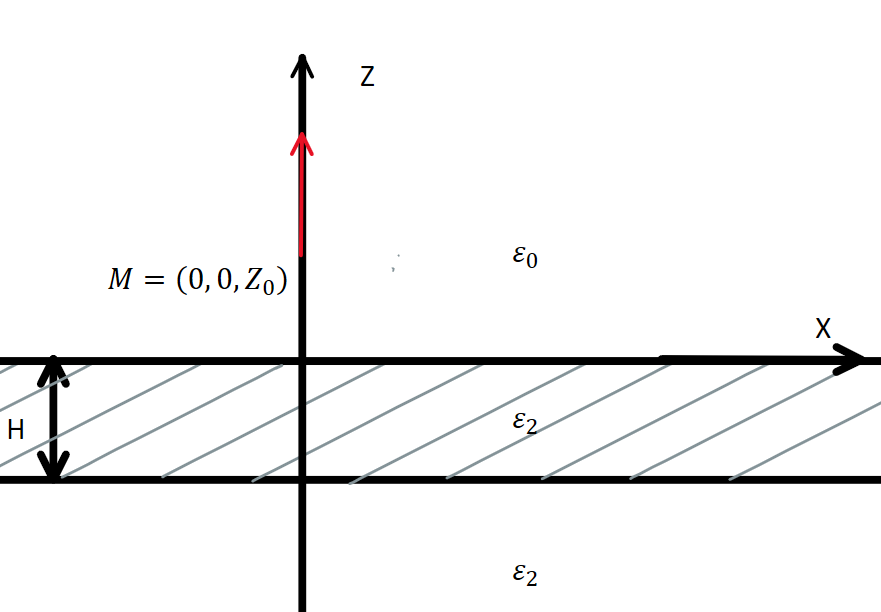
\includegraphics[width=0.5\textwidth]{Рис 2.PNG} % Вставка изображения. Укажите путь к вашему изображению вместо example-image
		\caption{Плоскослоистая среда с вертикальным дипольным источником} % Подпись к рисунку
		\label{fig:example2} % Метка для ссылки на рисунок
	\end{figure}
	
	Рассмотрим случай когда у источника $\bar{j} = (0, 0, j_z)$ тогда (5.1) можно записать в виде:
	
	\begin{equation}
		\begin{cases}\Delta(A_x) + k^2 A_x = 0 \\ \Delta(A_y) + k^2 A_y = 0 \\ \Delta(A_z) + k^2 A_z = -j_z * \delta(M, M_0) \mu\end{cases}
	\end{equation}
	
	де $\delta(M, M_0)$ - функция Дирака т.е
	
	\begin{equation*}
		\delta(M, M_0) = \begin{cases} 1, M = M_0, \\ 0, иначе\end{cases} \\  \int \int \int f(M)\delta(M, P)dv_M = f(P)
	\end{equation*}
	
	Найдем условия для векторного потенциала что бы на $z = 0, z = h$ выполнялись (2.1)
	
	Пусть 
	\begin{equation}
		  A_x = A_y = 0, \Delta A_Z + k^2_1A_Z = -\delta(M, M_0)j_z \\
	\end{equation}
	
	и
	
	\begin{equation*}
		\tag{8.1} [A_z] = [\frac{\partial A_z}{k^2 \partial z}] = 0 
	\end{equation*}
	
	тогда $A=(0, 0, A_z) - решение (7)$
	
	Так как присутствует осевая симметрия, $A_z$  зависит только от $z, z_0, \rho = \sqrt{(x-x_0)^2 + (y - y_0)^2}$ тогда решение (8), (8.1) представимо в виде:
	
	\begin{equation}
		A_z(\rho, z, z_0) = \int_0^\infty J_0(\lambda \rho) w(\lambda, z, z_0)\lambda d\lambda \\
	\end{equation}
	
	При подстановке (9) в (8), $z \neq z_0$ получаем
	
	\begin{equation}
		 \int_0^\infty((\frac{\partial^2}{\partial x^2}J_0(\lambda \rho) + (\frac{\partial^2}{\partial y^2}J_0(\lambda \rho) )w(\lambda, z, z_0) + J_0(\lambda \rho)(\frac{\partial^2}{\partial z^2}w(\lambda, z, z_0) + k^2 w(\lambda, z, z_0)))\lambda d \lambda  = 0 \\ 
	\end{equation}
	
	Так как $\Delta_{x, y}J_0(\lambda, z, z_0) = -\lambda^2 J_0(\lambda \rho)$ то достаточно что при $z \neq z_0$ $w$ удовлетворяла:
	
	\begin{equation*}
		\tag{10.1} \frac{\partial^2}{\partial z^2}w(\lambda, z, z_0) + - (\lambda^2 - k^2) w(\lambda, z, z_0) = 0 \\ 	
	\end{equation*}
	
	В $M = M_0$ $A_z(\rho, z, z_0) $ имеет особенность вида $\frac{1}{R(M, M_0)}$, 
	
	кроме того если $\Delta U + k^2_1U= -\delta(M, M_0)$  - уравнение Гельмгольца,
	
	то
	\begin{equation}
		U = \frac{e^{ikR(M, M_0)}}{R(M, M_0)}
	\end{equation}
	
	
	в $M = M_0$ $U(\rho, z, z_0)$  имеет особенность вида $\frac{1}{R(M, M_0)}$ и справедливо представление:
	
	\begin{equation}
		\frac{e^{ik\sqrt{\rho^2 + (z - z_0)^2}}}{\sqrt{\rho^2 + (z - z_0)^2}} = \int_0^\infty J_0(\lambda \rho)\frac{e^{-\sqrt{\lambda^2 - k^2}|z - z_0|}}{\sqrt{\lambda^2 - k^2} }\lambda d \lambda \\ 	
	\end{equation}
	
	Функция $\frac{e^{-\sqrt{\lambda^2 - k^2}|z - z_0|}}{\sqrt{\lambda^2 - k^2} }$ непрерывна по z и имеет непрерывные производные при $z \neq z_0$ в 
	
	$z = z_0$  первая производная терпит разрыв = -2
	
	Тогда для того чтобы $A_z$ было решением (9) необходимо чтобы 
	
	\begin{equation}
		\begin{cases}
			\frac{\partial^2}{\partial z^2}w(\lambda, z, z_0) + - (\lambda^2 - k^2) w(\lambda, z, z_0) = 0$ \text{при} $z \neq z_0, \\
			\text{на границе:} [w] = [\frac{dw}{k^2dz}] = 0 \\
			
		\text{при} \space z = z_0 [w] = 0, \frac{dw}{k^2dz} = -2
		\end{cases}
	\end{equation}
	
	\subsection{Электромагнитное поле горизонтального диполя}
	
		\begin{figure}[h] % [h] означает, что рисунок будет размещен здесь, а не автоматически в конце раздела или страницы
		\centering % Выравнивание по центру
		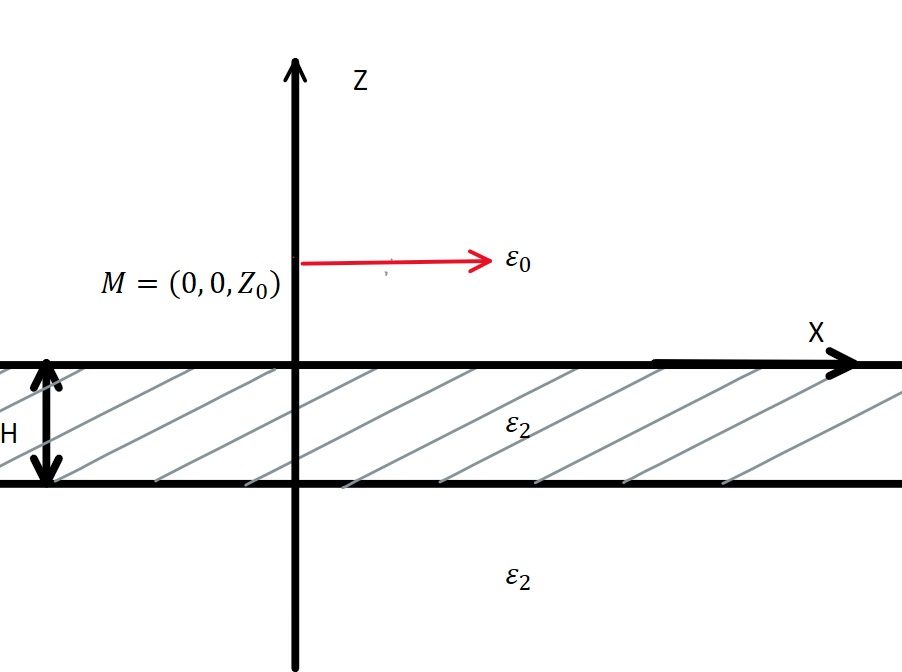
\includegraphics[width=0.5\textwidth]{Рис 3.PNG} % Вставка изображения. Укажите путь к вашему изображению вместо example-image
		\caption{Плоскослоистая среда с горизонтальным дипольным источником} % Подпись к рисунку
		\label{fig:example3} % Метка для ссылки на рисунок
	\end{figure}
	
	Рассмотрим случай когда у источника $\bar{j} = (j_x, 0, 0)$ тогда (5.1) можно записать в виде:
	
	\begin{equation}
		\begin{cases}\Delta(A_x) + k^2 A_x = -j_x \delta(M, M_0) \mu \\ \Delta(A_y) + k^2 A_y = 0  \\ \Delta(A_z) + k^2 A_z = 0\end{cases}
	\end{equation}
	
	\begin{equation}
		[A_x] = [A_y] = [A_z] = [\frac{\partial A_x}{\partial z}] = [\frac{\partial A_y}{\partial z}] = [\frac{1}{k^2}(\frac{\partial Ay}{\partial y} + \frac{\partial Ax}{\partial x} + \frac{\partial Az}{\partial z})] = 0 \\ 
	\end{equation}

	К сожалению решение в виде $A = (A_X, 0, 0)  $ искать нельзя тк необходимо выполнение условий
	
	\begin{equation}
		[A_x] = [\frac{\partial A_x}{\partial x}] = [\frac{\partial A_x}{k^2 \partial x}] = 0 \\ 
	\end{equation}
	
	Но эти условия не совместны.
	
	Поэтому будем искать решение в виде $A = (A_x, 0, A_z)$ и получается система
	
	\begin{equation}
		\begin{cases}\Delta(A_x) + k^2 A_x = -j_x \delta(M, M_0) \mu \\  A_y = 0  \\ \Delta(A_y) + k^2 A_z = 0\end{cases}
	\end{equation}
	
	\begin{equation}
		[A_x] = [A_z] = [\frac{\partial A_x}{\partial z}] = [\frac{1}{k^2}( \frac{\partial Ax}{\partial x} + \frac{\partial Az}{\partial z})] = 0 \\ 
	\end{equation}
	
	Так же должны выполняться условия излучения
	
	\begin{equation*}
		\begin{cases}
			A_x = O_{r \rightarrow \infty} (\frac{1}{r}) \\ 
			\frac{\partial A_x}{\partial r} + i k A_x = o(\frac{1}{r})\\
			A_z = O_{r \rightarrow \infty} (\frac{1}{r}) \\ 
			\frac{\partial A_z}{\partial r} + i k A_z = o(\frac{1}{r})
		\end{cases}
	\end{equation*}
	
	Теперь ищем векторные потенциалы в виде:
	\begin{equation}
		A_x(\rho, z, z_0) = \int_0^\infty J_0(\lambda \rho) u(\lambda, z, z_0)\lambda d\lambda \\ 
	\end{equation}
	
	\begin{equation}
		A_z(\rho, z, z_0) = \int_0^\infty J_0(\lambda \rho) (g(\lambda, z, z_0) - \frac{du(\lambda, z, z_0)}{dz})\lambda d\lambda \\ 
	\end{equation}
	
	Подставив (19) в (17), требуя условия (18) , получим, что достаточно чтобы для $\forall \lambda, z \neq z_0\ $ было выполнено:
	
	\begin{equation}
		\frac{\partial^2}{\partial z^2}u(\lambda, z, z_0) + - (\lambda^2 - k^2) u(\lambda, z, z_0) = 0,
		 \newline
		  [{u}]  = [\frac{\partial u}{\partial z}] = 0 
	\end{equation}
	
	и при $z = z_0$:
	
	\begin{equation}
		[{u}] = 0, \space  [\frac{du}{dz}] = -2\\
	\end{equation}
	
	Теперь подставим (20) в (17) 
	
	\begin{equation}
		\begin{aligned}
			\Delta_{x, y} \frac{\partial}{\partial x}\int_0^\infty J_0(\lambda \rho) (g(\lambda, z, z_0) - \frac{du(\lambda, z, z_0)}{dz}\frac{d \lambda}{ 	\lambda} + \\ \frac{\partial^2}{\partial z^2} \frac{\partial}{\partial x}\int_0^\infty J_0(\lambda \rho) (g(\lambda, z, z_0) - \frac{du(\lambda, z, z_0}{dz} \frac{d \lambda}{\lambda} + \\    k^2\frac{\partial}{\partial x}\int_0^\infty J_0(\lambda \rho) (g(\lambda, z, z_0) - \frac{du(\lambda, z, z_0)}{dz}) \frac{d \lambda}{\lambda} = 0              
		\end{aligned}
	\end{equation}
	
	\newpage
	
	Уравнение выше сводится к:
	
	\begin{equation}
		\begin{aligned}
			\frac{\partial}{\partial x} \int_0^\infty J_0(\lambda \rho)\frac{d}{dz}((\lambda^2 - k^2)u(\lambda, z, z_0) - \frac{d^2 u(\lambda, z, z_0)}{dz^2})\frac{d\lambda}{\lambda} + \\ \frac{\partial}{\partial z} \int_0^\infty J_0(\lambda \rho) \frac{(d^2g(\lambda, z, z_0)}{dz^2} - (\lambda^2 - k^2)g(\lambda, z, z_0))\frac{d \lambda}{\lambda} = 0 
		\end{aligned}
	\end{equation}
	
	Для выполнения (24) достаточно чтобы g удовлетворяла:
	
	\begin{equation}
		\frac{d^2 g(\lambda, z, z_0)}{d z^2} - (\lambda^2 - k^2)g(\lambda, z, z_0) = 0 
	\end{equation}
	
	Для выполнения (18) достаточно (для непрерывности $A_z$) чтобы:
	
	\begin{equation}
		\begin{aligned}
			[g(\lambda, z, z_0 - \frac{du(\lambda, z, z_0)}{dz}] = 0 \\ [u] = 0 \\ [\frac{du}{dz}] = -2 \\ 
		\end{aligned}
	\end{equation}
	
	Подставив в $ [\frac{1}{k^2}( \frac{\partial Ax}{\partial x} + \frac{\partial Az}{\partial z})] = 0$ (19), (20)  получим:
	
	\begin{equation}
		\begin{aligned}
			[\frac{1}{k^2}\frac{\partial}{\partial x} \int_0^\infty J_0(\lambda \rho) (\lambda^2u(\lambda, z, z_0) + \frac{dg(\lambda, z, z_0)}{dz} - \frac{d^2 u(\lambda, z, z_0)}{d z^2}) \frac{d\lambda}{\lambda}] = 0 \\                                   [\frac{\partial}{\partial x} \int_0^\infty J_0(\lambda \rho) (u(\lambda, z, z_0) + \frac{1}{k^2} \frac{dg(\lambda, z, z_0}{dz})\frac{d\lambda}{\lambda}] = 0 \\ 
		\end{aligned}
	\end{equation}
	
	$[u] = 0$ из  (26) поэтом для  $[\frac{1}{k^2}( \frac{\partial Ax}{\partial x} + \frac{\partial Az}{\partial z})] = 0$ достаточно  $[\frac{1}{k^2}( \frac{dg(\lambda, z, z_0)}{dz})] = 0$
	
	Уравнения для $A_z$ - уравнение Гельмгольца,
	то достаточно чтоб g была решением и удовлетворяла условиям на границе.
	
	\begin{equation}
		\begin{cases}\frac{d^2 g(\lambda, z, z_0)}{d z^2} - (\lambda^2 - k^2)g(\lambda, z, z_0) = 0  \\  [\frac{1}{k^2}( \frac{dg(\lambda, z, z_0)}{dz})] = 0 \\ [g(\lambda, z, z_0)] = 0 \\ z \neq z_0 \end{cases} \\ 
	\end{equation}
	
	Если для g выполнены условия излучения, то и для векторного потенциала тоже.
	
	В $z = z_0$:
	
	\begin{equation}
		\begin{aligned}
			[g(\lambda, z, z_0)] = - 2 \\ [\frac{1}{k^2}( \frac{dg(\lambda, z, z_0)}{dz})] = 0 \\ 
		\end{aligned}
	\end{equation}
	
	Для переменной y - аналогично
	
	\subsection{Тензор Грина электрического типа}
	
	Для плоскопараллельной слоистой среды тензор Грина для
	векторного потенциала имеет следующий вид
	
	\begin{equation}
		G_A(M, M_0) = \begin{pmatrix} G_1(M, M_0) & 0 & 0 \\            0 & G_1(M, M_0) & 0 \\ \frac{\partial}{\partial x}G_2(M, M_0) & \frac{\partial}{\partial y}G_2(M, M_0) & G_3(M, M_0)\end{pmatrix} 
	\end{equation}
	
	Элементы тензора Грина для векторного потенциала можно найти путем вычисления
	преобразования Ханкеля от решений трёх краевых задач для обыкновенных
	дифференциальных уравнений второго порядка с кусочно-постоянными
	коэффициентами.
	
	\begin{equation}
		\begin{aligned}
			G_1(M, M_0) = \int_0^\infty J_0(\lambda \rho) u(\lambda, z, z_0)\lambda d \lambda  \\ G_2(M, M_0) = \int_0^\infty J_0(\lambda \rho) (g(\lambda, z, z_0) - \frac{du(\lambda, z, z_0)}{dz})\lambda d \lambda \\ G_3(M, M_0) = \int_0^\infty J_0(\lambda \rho) w(\lambda, z, z_0)\lambda d \lambda 
		\end{aligned}
	\end{equation}
	
	\begin{equation}
		\begin{matrix} \text{Дифференциальное} \space 
			\text{уравнение} & \text{Условия} \space\text{на} \space\text{границах} &  \text{Условие} \space \text{при} \space z = z_0 \\ \frac{d^2w}{dz^2} - (\lambda^2 - k^2)w = 0 & [w] = [\frac{dw}{k^2dz}]=0 & [w] = 0, [\frac{dw}{k^2dz}]=-2 \\ \\ \frac{d^2u}{dz^2} - (\lambda^2 - k^2)u = 0 & [u] = [\frac{du}{dz}] = 0 & [u] = 0, [\frac{du}{dz}] = -2 \\ \\ \frac{d^2g}{dz^2} - (\lambda^2 - k^2)g = 0 &  [g] = [\frac{dg}{k^2dz}]=0 & [g] = [\frac{dg}{k^2dz}]=-2\end{matrix} \space 
	\end{equation}
	
	\subsection{Решение краевой задачи для функции u}
	
	Из условий излучения следует, что $u(\lambda, z, z_0) \space при \space z>0$  имеет вид
	
	\begin{equation}
		u(\lambda, z , z_0) = a e^{-\eta_0 z} + \frac{e^{-\eta_0 |z - z_0|}}{\eta_0} 
	\end{equation}
	
	$a - const, а \space \frac{e^{-\eta_0|z - z_0|}}{\eta_0}$ обеспечивает выполнение $[u] = 0, [\frac{du}{dz}] = -2 \space при \space z = z_0$
	Общее решение уравнения для $u(\lambda, z, z_0) \space при \space z_1<z<0$ имеет вид
	
	\begin{equation}
		u_1(\lambda, z, z_0) = a_1(e^{\eta_1(z - z_1)} + r_1e^{-\eta_1z}), \space a_1, r_1 -const 
	\end{equation}
	
	В случае $z<z_1:$
	
	\begin{equation}
		u_2(\lambda, z, z_0) = a_2(e^{\eta_2(z - z_1)}), a_2-const 
	\end{equation}
	
	
	Коэффициенты $a, a_1, a_2, r_1$ найдем из граничных условий
	Пусть $\eta_j = \sqrt{\lambda^2 - k^2_j}, j = 0, 1, 2$
	
	\begin{equation}
		\begin{aligned}
			r_1 = \frac{\eta_1 - \eta_2}{\eta_1 + \eta_2}e^{\eta_1z_1}, z = z_1 \\ (a_2 - a_1) = \frac{\eta_1 - \eta_2}{\eta_1 + \eta_2}
		\end{aligned}
	\end{equation}
	
	\begin{equation}
		a= (-1 + \frac{2 \eta_0(1+r_1e^{\eta_1z_1})}{\eta_0(1+r_1e^{\eta_1 z_1}) + \eta_1(1 - r_1e^{\eta_1 z_1})})\frac{e^{-\eta_0z_0}}{\eta_0}, z = 0 
	\end{equation}
	
	
	\begin{equation}
		r_0 = -1 + \frac{2 \eta_0(1+r_1e^{\eta_1z_1})}{\eta_0(1+r_1e^{\eta_1 z_1}) + \eta_1(1 - r_1e^{\eta_1 z_1})}\tag{37.1}
	\end{equation}
	
	Из (37)  и (33) следует что в $z>0$:
	
	\begin{equation}
		u(\lambda, z, z_0)  = \frac{e^{\eta_0|z-z_0|}}{\eta_0} + r_0 \frac{e^{-\eta_0(z_0+z)}}{\eta_0} 
	\end{equation}
	
	Или обозначив
	
	\begin{equation}
		\begin{aligned}
			\begin{cases} f_0(\lambda, z, z_0) = \frac{e^{\eta_0|z-z_0|}}{\eta_0} + \frac{e^{-\eta_0(z_0+z)}}{\eta_0} \\  \\ f_u(\lambda) = \frac{2 (1+r_1e^{\eta_1z_1})}{\eta_0(1+r_1e^{\eta_1 z_1} + \eta_1(1 - r_1e^{\eta_1 z_1})} \end{cases} 
		\end{aligned}
	\end{equation}
	
	Получим что $u(\lambda, z, z_0)$  представима в виде:
	
	\begin{equation}
		u(\lambda, z, z_0) = f_0(\lambda, z, z_0) + e^{-\eta_0(z_0 + z)}f_u(\lambda) 
	\end{equation}
	
	Для функций $w, g $ введем дополнительную фиктивную границу $z = z_0$ тогда:
	
	%%тут нужна картинка
	
	Тогда аналогично функции u получим
	
	\begin{equation}
		\begin{aligned}
			w(\lambda, z, z_0) = f_0(\lambda, z, z_0) + e^{-\eta_0(z_0 + z)}f_w(\lambda) \\ f_w(\lambda) = \frac{2 \varepsilon_1(1+r_1e^{\eta_1z_1})}{\varepsilon_0 \eta_0(1+r_1e^{\eta_1 z_1}) + \varepsilon_0\eta_1(1 - r_1e^{\eta_1 z_1})}  
		\end{aligned}
	\end{equation}
	
	\begin{equation}
		\begin{aligned}
			g(\lambda, z, z_0) - \frac{du(\lambda, z, z_0)}{dz} = (R_0 + r_0)e^{-\eta_0(z_0+ z)} \\ R_0 = -1 + \frac{2 \varepsilon_1\eta_0(1+r_1e^{\eta_1z_1})}{\varepsilon_1\eta_0(1+r_1e^{\eta_1 z_1}) + \varepsilon_0\eta_1(1 - r_1e^{\eta_1 z_1})}
		\end{aligned}
	\end{equation}
	
	Подставив вычисленные функции в искомый тензор Грина для векторного потенциала получим:
	
	\begin{equation}
		\begin{aligned}
			G_1(M, M_0) = \int^\infty_0 J_0(\lambda \rho) f_0(\lambda, z, z_0) \lambda d \lambda + \\ \int^\infty_0J_0(\lambda \rho)e^{-\eta_0(z_0 + z)}f_u(\lambda) \lambda d \lambda 
		\end{aligned}
	\end{equation}
	
	
	\begin{equation}
		\begin{aligned}
			G_3(M, M_0) = \int^\infty_0 J_0(\lambda \rho) f_0(\lambda, z, z_0) \lambda d \lambda + \\ \int^\infty_0J_0(\lambda \rho)e^{-\eta_0(z_0 + z)}f_w(\lambda) \lambda d \lambda 
		\end{aligned}
	\end{equation}
	
	\begin{equation}
		\begin{aligned}
			G_2(M, M_0) = \int_0^\infty J_0(\lambda\rho)(R_0(\lambda) + r_0(\lambda))e^{-\eta_0(z_0 + z)} \frac{d \lambda}{\lambda} \\ \frac{\partial G_2(M, M_0)}{\partial y} = \frac{-y - y_0}{\rho} \int_0^\infty J_1(\lambda\rho)(R_0(\lambda) + r_0(\lambda))e^{-\eta_0(z_0 + z)} {d \lambda} \\ \frac{\partial G_2(M, M_0)}{\partial x} = \frac{-x - x_0}{\rho} \int_0^\infty J_1(\lambda\rho)(R_0(\lambda) + r_0(\lambda))e^{-\eta_0(z_0 + z)} {d \lambda} 
		\end{aligned}
	\end{equation}
	
	\begin{equation*}
		\begin{aligned}
			G_A(M, M_0) =
			 \begin{pmatrix} G_1(M, M_0) & 0 & 0 \\  
				   0 & G_1(M, M_0) & 0 \\ 
				   \frac{\partial}{\partial x}G_2(M, M_0) & \frac{\partial}{\partial y}G_2(M, M_0) & G_3(M, M_0) \\
			\end{pmatrix} \\	
		\end{aligned}
		\tag{30}
	\end{equation*}
	
	\newpage
	
	\section{Электромагнитное поле диполя в плоскослоистой среде с графеновым  слоем}
	
	\subsection{Постановка задачи}
	
	Дана плоскослоистая среда состоящая из 2х слоев с различными проводимостями $$\varepsilon_1, \varepsilon_2 - const, $$разделенных слоем графена. 
	В точке $M_s(0,0,z_s) $ находится источник электромагнитного поля - электрический диполь, его поле изменяется во времени по закону $e^{-i\omega t}$.
	
	\begin{figure}[h] % [h] означает, что рисунок будет размещен здесь, а не автоматически в конце раздела или страницы
		\centering % Выравнивание по центру
		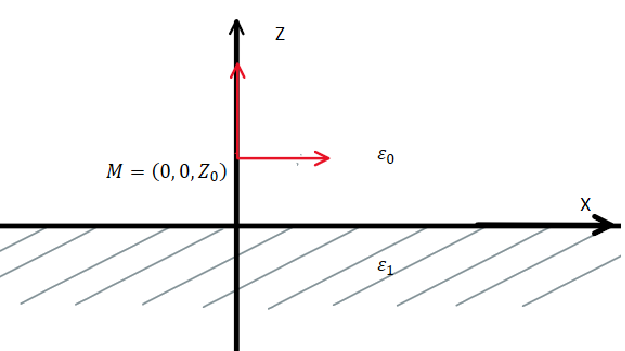
\includegraphics[width=0.5\textwidth]{Рис 6.PNG} % Вставка изображения. Укажите путь к вашему изображению вместо example-image
		\caption{Плоскослоистая среда с графеновым слоем} % Подпись к рисунку
		\label{fig:example6} % Метка для ссылки на рисунок
	\end{figure}
	
	Тогда система уравнений Максвелла имеет вид:
	
	
	\begin{equation}
		\begin{cases} rot \vec{H} = -i \omega \varepsilon \vec{E} + j_{ст} \\ rot \vec{E} = iw\mu \vec{H} \end{cases}
	\end{equation}
	
	На обеих границах выполняются условия непрерывности касательных компонент полей-
	
	\begin{equation}
		\begin{cases}
			 [n \times E ]_S = 0, \\
			 [n \times H]_S = \delta E_{\tau} 
		\end{cases}
	\end{equation}
	
	где $\delta = \delta_1 + \delta_2 * {|E_{\tau}|}^2$, где $\delta_2 \approx 0$.
	
	
	Введем 2 векторных потенциала - $A$ и $a$ с калибровками Лоренца:
	
	$$\begin{cases}
		\vec{E} = \vec{E^{*}} + \vec{E^{**}} \\
		\vec{E} = \vec{H^{*}} + \vec{H^{**}}
	\end{cases}$$
		
	\begin{equation}
		\begin{cases}
			\vec{H^*_{1, 2}} = \frac{k^2_{1, 2}a}{\mu_0} + \frac{grad div \vec{a}}{\mu_0}  \\
			\vec{E^*_{1, 2}} = i \omega rot \vec{a}
		\end{cases}
	\end{equation}
	
	\begin{equation}
		\begin{cases}
			\vec{H^{**}_{1, 2}} = \frac{rot \vec{A}}{\mu_0} \\
			\vec{E^{**}_{1, 2}} = i \omega \vec{A} + grad(\frac{i \omega}{k^2_{1, 2}} div \vec{A}) \\
		\end{cases}
	\end{equation}
	
	Граничные условия (47) можно переписать в виде:
	
	\begin{equation*}
		\tag{47.1}
		\begin{cases}
			[E_x] = 0 \\
			[E_y] = 0 \\
			[H_x] = \delta E_{x_1} \\
			[H_y] = \delta E_{y_1}
			
		\end{cases}
	\end{equation*}
	
	\subsection{Вертикальный диполь}
	
	Подставив (48, 49) в (47.1) получим в $z = 0$:
	
	\begin{equation}
		\begin{cases}
			\frac{1}{k_1^2} \frac{\partial A_{z_1}}{\partial z} = \frac{1}{k_2^2} \frac{\partial A_{z_2}}{\partial z} \\
			
			a_{z_1} = a_{z_2} \\
			
			-\frac{\partial A_{z_2}}{\partial x} + \frac{\partial^2 a_{z_2}}{\partial y \partial z} + \frac{\partial A_{z_1}}{\partial x} - \frac{\partial^2 a_{z_1}}{\partial y \partial z} = i \omega \delta (\frac{1}{k_1^2} \frac{\partial^2 A_{z_1}}{\partial y \partial z} - \frac{\partial a_{z_1}}{\partial x}) \\
			
			\frac{\partial A_{z_2}}{\partial y} + \frac{\partial^2 a_{z_2}}{\partial x \partial z} - \frac{\partial A_{z_1}}{\partial y} - \frac{\partial^2 a_{z_1}}{\partial x \partial z} = i \omega \delta (\frac{1}{k_1^2} \frac{\partial^2 A_{z_1}}{\partial x \partial z} + \frac{\partial a_{z_1}}{\partial y})
			
			
		\end{cases}
	\end{equation}
	
	
	так как 
	
	\begin{equation}
		\begin{aligned}
			H_x = \frac{1}{\mu_0} (\frac{\partial ^ 2 a_z}{\partial x \partial z} + \frac{\partial A_z}{\partial y}) \\
			H_y = \frac{1}{\mu_0} (\frac{\partial ^ 2 a_z}{\partial y \partial z} - \frac{\partial A_z}{\partial x}) \\
			E_x = i \omega \delta (\frac{1}{k_1^2} \frac{\partial^2 A_{z_1}}{\partial y \partial z} - \frac{\partial a_{z_1}}{\partial x}) \\			
			E_y = i \omega \delta (\frac{1}{k_1^2} \frac{\partial^2 A_{z_1}}{\partial x \partial z} + \frac{\partial a_{z_1}}{\partial y})
		\end{aligned}
	\end{equation}
	
	при $z \neq z_0$ $A_z$ и $a_z$ удовлетворяют 
	
	\begin{equation}
		\begin{aligned}
			\Delta A_z + k^2 A_z = 0 \\
			\Delta a_z + k^2 a_z = 0
		\end{aligned}
	\end{equation}
	
	при приближении к источнику должно выполняться:
	
	\begin{equation}
		A_z \rightarrow \frac{M}{4 \pi} \frac{\exp{i k_1 R}}{R} 
	\end{equation}
	
	где, $R = \sqrt{x^2 + y^2 + {(z - z_0)} ^ 2}$.
	
	при $R \rightarrow \infty$ выполняются
	
	\begin{equation}
		\begin{cases}
			A_z = O_{R \rightarrow \infty}(\frac{1}{R}) \\
			\frac{\partial A_z}{\partial R} + i A_z k = o_{R \rightarrow \infty}(\frac{1}{R})
		\end{cases}
	\end{equation}
	
	Будем искать решение в виде преобразований Ханкеля (аналогично случаю без графена)
	
	\begin{equation}
		\begin{aligned}
			a_z = \frac{I \mu_0 }{4 \pi} \int_0^{\infty} X J_0(mz)dm \\
			A_z = \frac{I \mu_0 }{4 \pi} \int_0^{\infty} V J_0(mz)dm
		\end{aligned}
	\end{equation}
	
	тогда $X$ и $V$ удовлетворяют
	
	\begin{equation}
		\begin{aligned}
			\frac{\partial^2 X}{\partial z^2} - n_{1, 2}^2 X = 0 \\
			\frac{\partial^2 V}{\partial z^2} - n_{1, 2}^2 V = 0 \\
		\end{aligned}
	\end{equation}
	
	где $n_{1, 2}^2 = m^2 - k_{1, 2}^2$, $Re (n) > 0$
	
	\begin{equation*}
		\tag{50.1}
		\begin{aligned}
			& \frac{1}{k_1^2} \frac{\partial A_{z_1}}{\partial z} = \frac{1}{k_1^2} \frac{\partial A_{z_2}}{\partial z} \\
			&a_{z_1} = a_{z_2} \\
			& A_{z_2} - A_{z_1} = i \omega \delta a_{z_1} \\
			&\frac{\partial a_{z_2}}{\partial z} - \frac{\partial a_{z_1}}{\partial z} = -i \omega \delta \frac{1}{k_1^2} \frac{\partial A_{z_1}}{\partial z} \\ 
		\end{aligned}
	\end{equation*}
	
	для $X$ и $V$ получим в $z = 0$:
	
	\begin{equation}
		\begin{aligned}
			& \frac{1}{k_1^2} \frac{\partial V_1}{\partial z} = \frac{1}{k_1^2} \frac{\partial V_2}{\partial z} \\
			&X_1 = X_2 \\
			& V_2 - V_1 = i \omega \delta X_2 \\
			&\frac{\partial X_2}{\partial z} - \frac{\partial X_1}{\partial z} = -i \omega \delta \frac{1}{k_2^2} \frac{\partial V_2}{\partial z} \\ 
		\end{aligned}
	\end{equation}
	\newpage
	в $z = z_0$
	
	
	\begin{equation}
		\begin{aligned}
			&\frac{\partial X_1^*}{\partial z} = \frac{\partial X_1}{\partial z} \\
			&X_1^* = X_1 \\
			&\frac{\partial V_1^*}{\partial z} - \frac{\partial V_1}{\partial z} = 2 \\
			&V_1^* = V_1 \\
		\end{aligned}
	\end{equation}
	
	Будем искать $V_1, V_2, V_1^*, X_1, X_2$ в виде:
	
	\begin{equation}
		\begin{aligned}
			&V: \\
			& z > z_0 \space 	&V_1^* = \beta_1^* e^{-n_1z} \\
			& z_0 > z > 0 \space	 &V_1 = \beta_1 e^{-n_1z} + \gamma_1 e^{n_1z} \\
			& z < 0 \space	&V_2 =  \gamma_2 e^{n_2z} \\
			&X: \\
			& z > 0 \space	&X_1 = d_1 e^{-n_1z} \\
			& z < 0	\space	&X_2 = c_2 e^{n_2z} 
		\end{aligned}
	\end{equation}

	Имеем 6 уравнений и 6 коэффициентов - решаем:

	\begin{equation}
		\begin{aligned}
			&\gamma_1 = \frac{e^{-n_1z_0}}{n_1} \\
			&\beta_1^* = \beta_1 - \frac{e^{n_z0}}{n_1} \\
			&L = -\frac{n_1 k_2^2}{n_2 k_1^2} + \frac{D^2 n_1}{(n_1 + n_2)k_1^2} \\
			&\beta_1 = \frac{e^{-n_1 z_0}}{n_1} (-1 + \frac{2L}{1 + L}) \\
			&\gamma_2 = \frac{k_2^2}{k_1^2} \frac{e^{-n_1z_0}}{n_2}(2 - \frac{D^2 n_1}{(n_1 + n_2)k_1^2}) \\
			&d_1 = c_1 = \frac{D e^{-n_1 z_0}}{(n_1 + n_2) k_1^2}(2 - \frac{D^2 n_1}{(n_1 + n_2)k_1^2}) \\ 
		\end{aligned}
	\end{equation}
	
	\newpage
	
	\subsection{Горизонтальный диполь}
	
	Для горизонтального диполя получим шраничные условия при $z = 0$:
	
	\begin{equation}
		\begin{cases}
			A_{x_1} = A_{x_2} \\
			A_{y_1} = A_{y_2} \\
			\frac{\partial A_{x_2}}{\partial z} - \frac{\partial A_{x_1}}{\partial z} = i \omega \delta A_{y_1} \\
			\frac{\partial A_{y_2}}{ \partial z} - \frac{\partial A_{y_1}}{\partial z} = i \omega \delta A_{x_1} \\
			a_{z_1} = a_{z_2} \\
			\frac{div(\vec{A_1})}{k_1^2} = \frac{div(\vec{A_2})}{k_2^2} \\
			A_{z_2} - A_{z_1} = i \omega \delta a_{z_1} \\
			\frac{\partial a_{z_2}}{\partial z} - \frac{\partial a_{z_1}}{\partial z} = i \omega \delta \frac{div(\vec{A_1})}{k_1^2}
		\end{cases}
	\end{equation}
	
	Так же вблизи источника выполняется:
	\begin{equation}
		A_x \rightarrow \frac{I \mu_0}{4 \pi} \frac{e^{i k_1 R}}{R}
	\end{equation}
	
	Представим $A_z$ и $a_z$ в виде:
	\begin{equation}
		\begin{aligned}
			A_z = \frac{\partial \text{П}}{\partial x} + \frac{\partial T}{\partial y} \\
			a_z = \frac{\partial P}{\partial x} + \frac{\partial Q}{\partial y} \\
		\end{aligned}
	\end{equation}
	
	тогда последние 2 условия из 61 можно переписать в виде:
	
	\begin{equation}
		\begin{aligned}
			&\frac{\partial \text{П}_2}{\partial x} - \frac{\partial \text{П}_1}{\partial x} + \frac{\partial T_2}{\partial y} - \frac{\partial T_1}{\partial y} = i \omega \delta (\frac{\partial P_1}{\partial x} + \frac{\partial Q_1}{\partial y}) \\
			&\frac{\partial^2 P_2}{\partial x \partial z} - \frac{\partial^2 P_1}{\partial x \partial z} + \frac{\partial^2 Q_2}{\partial y \partial z} - \frac{\partial^2 Q_1}{\partial y \partial z} = \frac{i \omega \delta}{k_1^2} (\frac{\partial A_{x_1}}{\partial x} + \frac{\partial A_{y_1}}{\partial y} + \frac{\partial^2 \textit{П}_1}{\partial x \partial z} + \frac{\partial ^ 2 T_1}{\partial y \partial z} )
		\end{aligned}
	\end{equation} 
	
	Для выполнения (64) достаточно системы:
	
	\begin{equation}
		\begin{cases}
			\text{П}_2 - \text{П}_1 = i \omega \delta P_1 \\
			\frac{\partial P_2}{\partial z} - \frac{\partial P_1}{\partial z} = \frac{i \omega \delta}{k_1^2} (A_{x_1} + \frac{\partial \text{П}_1}{\partial z}) \\
			T_2 - T_1 = i \omega \delta Q_1 \\
			\frac{\partial Q_2}{\partial z} - \frac{\partial Q_1}{\partial z} = \frac{i \omega \delta}{k_1^2} (A_{y_1} + \frac{\partial T_1}{\partial z}) \\
 		\end{cases}
	\end{equation}
	
	\newpage
	
	так как:
	
	\begin{equation*}
		\begin{aligned}
			&a_{z_1} = a_{z_2} \\ 
			&\frac{div(\vec{A_1})}{k_1^2} = \frac{div(\vec{A_2})}{k_2^2} \\
		\end{aligned}
	\end{equation*}
	
	получаем 
	\begin{equation*}
		\tag{65.1}
		\begin{cases}
			P_1 = P_2 \\
			\frac{1}{k_1^2}(A_{x_1} + \frac{\partial \text{П}_1}{\partial z}) = \frac{1}{k_2^2}(A_{x_2} + \frac{\partial \text{П}_2}{\partial z}) \\
			Q_1 = Q_2 \\
			\frac{1}{k_1^2}(A_{y_1} + \frac{\partial T_1}{\partial z}) = \frac{1}{k_2^2}(A_{y_2} + \frac{\partial T_2}{\partial z})
		\end{cases}
	\end{equation*}
	
	Систему из 8 уравнений можно разбить на две независмые системы сожержащие $P, \text{П}, A_x$ и $T, Q, A_y$
	так же отдельно можем вычислить $A_x$ и $A_y$ из 61 и 62.
	
	Рассмотрим систему:
	
	\begin{equation}
		\begin{cases}
			P_1 = P_2 \\
			\frac{1}{k_1^2}(A_{x_1} + \frac{\partial \text{П}_1}{\partial z}) = \frac{1}{k_2^2}(A_{x_2} + \frac{\partial \text{П}_2}{\partial z}) \\
			\text{П}_2 - \text{П}_1 = i \omega \delta P_1 \\
			\frac{\partial P_2}{\partial z} - \frac{\partial P_1}{\partial z} = \frac{i \omega \delta}{k_1^2} (A_{x_1} + \frac{\partial \text{П}_1}{\partial z}) \\
		\end{cases}
	\end{equation}
	
	Будем искать $P, A_x, \text{П}$ в виде преобразований Ханкеля
	
	\begin{equation}
		\begin{aligned}
			& \text{П} = \frac{I \mu_0}{4 \pi} \int_0^{\infty} M J_0(mz) dm \\
			& P = \frac{I \mu_0}{4 \pi} \int_0^{\infty} N J_0(mz) dm \\
			& A_x = \frac{I \mu_0}{4 \pi} \int_0^{\infty} L J_0(mz) dm \\
			& A_y = \frac{I \mu_0}{4 \pi} \int_0^{\infty} S J_0(mz) dm \\
			& Q = \frac{I \mu_0}{4 \pi} \int_0^{\infty} K J_0(mz) dm \\
			& T = \frac{I \mu_0}{4 \pi} \int_0^{\infty} D J_0(mz) dm \\
		\end{aligned}
	\end{equation} 
	
	тогда систему, полученную из замены и уравнений Масвела:
	
	\begin{equation}
		\begin{cases}
			\Delta A_x + k^2 A_x = 0 \\
			\Delta A_y + k^2 A_y = 0 \\
			\Delta A_z + k^2 A_z = 0 \\
			\Delta a_z + k^2 a_z = 0 \\
		\end{cases}
	\end{equation}
	
	можно заменить достаточной:
	
	\begin{equation}
		\begin{cases}
			 \frac{\partial \Delta M}{\partial x} + n^2 \frac{\partial M}{\partial x} = 0 \\
			 \frac{\partial \Delta N}{\partial x} + n^2 \frac{\partial N}{\partial x} = 0 \\
			 \frac{\partial \Delta K}{\partial y} + n^2 \frac{\partial K}{\partial y} = 0 \\
			 \frac{\partial \Delta D}{\partial y} + n^2 \frac{\partial D}{\partial y} = 0 \\
			 \Delta L + n^2 L = 0 \\
			 \Delta S + n^2 S = 0 \\
		\end{cases}
	\end{equation}
	
	где $n^2 = m^2 - k^2$.
	
	Для $M, N$ решения представимы в виде:
	
	\begin{equation}
		\begin{aligned}
			&V: \\
			& z > 0 \space 	&M_1 = x\alpha_1 e^{-n_1z} \\
			& z < 0 \space	&M_2 = x\alpha_2 e^{n_2z} \\
			&X: \\
			& z > 0 \space	&N_1 = x\beta_1 e^{-n_1z} \\
			& z < 0	\space	&N_2 = x\beta_2 e^{n_2z} 
		\end{aligned}
	\end{equation}
	
	Коефициенты можно посчитать по следующим формулам:
	
	\begin{equation}
		\begin{aligned}
			&\alpha_1 = \frac{\frac{L_1(0)}{k_1^2} - \frac{L_2(0)}{k_2^2} + \frac{\omega^2 L_1(0)}{k_1^4 (n_2 - n_1)}}{x(\frac{n_2}{k_1^2} + \frac{n_1}{k_1^2} + \frac{\omega n_1 \delta}{k_1^4 (n_2 - n_1)})} \\
			&\beta_1 = \beta_2 = \frac{i \omega (L_1(0) - \alpha_1 n_1 x) \delta}{k_1^2 x (n_2 - n_1)} \\
			&\alpha_2 = \alpha_1 = i \omega \delta \beta_1		
		\end{aligned}
	\end{equation}
	
	аналогично для $K, D$.
	
	Далее вычислим коефициенты для $L, S$:
	
	\begin{equation}
		\begin{aligned}
			&L: \\
			& z > z_0 \space 	&L_3 = \gamma_1^* e^{-n_1z} \\
			& z_0 > z > 0 \space	 &L_1 = \kappa_1 e^{-n_1z} + \kappa_2 e^{n_1z} \\
			& z < 0 \space	&L_2 =  \gamma_2 e^{n_2z} \\
			&S: \\
			& z > 0 \space	&S_1 = d_1 e^{-n_1z} \\
			& z < 0	\space	&S_2 = d_2 e^{n_2z} 
		\end{aligned}
	\end{equation}
	
	при условии, что  при $z = 0$:
	
	\begin{equation}
		\begin{aligned}
			&L_1 = L_2 \\
			&S_1 = S_2 \\
			&\frac{\partial L_2}{\partial z} - \frac{\partial L_1}{\partial z} = i \omega \delta S_1 \\
			&\frac{\partial S_2}{\partial z} - \frac{\partial S_1}{\partial z} = i \omega \delta L_1 \\
		\end{aligned}
	\end{equation}
	
	а из особенности $A_x$ в $z = z_0$:
	
	\begin{equation}
		\begin{aligned}
			&\frac{\partial L_1}{\partial z} - \frac{\partial L_3}{\partial z} = 2 \\
			&L_1 = L_3 \\
		\end{aligned}
	\end{equation}
	
	тогда получим:
	
	\begin{equation}
		\begin{aligned}
			&\kappa_2 = \frac{e^{-n_1 z_0}}{n_1} \\
			&\gamma_1 = \kappa_1 - \frac{e^{n z_0}}{n_1} \\
			&\kappa_1 = - \frac{{(n_1 + n_2)}^2 + \omega^2 \delta^2}{n_1^2 - n_2^2 + \omega^2 \delta^2} \kappa_2 \\
			&d_1 = d_2 = \frac{\kappa_1 + \kappa_2}{n_1 + n_2} i \omega \delta \\
			&\gamma_2 = \kappa_1 + \kappa_2
		\end{aligned}
	\end{equation}
	
	
	\newpage
	
	\section{Плоская электромагнитная волна в плоскослоистой среде с графеновым слоем}
	
	Рассмотрим падение плоской электромагнитной волны под углом $\phi$ к нормали, на графеновый слой разделяющий две среды с известными коефициентами $\mu_1, \mu_2, \varepsilon_1, \varepsilon_2$.
	
	введем:
	
	\begin{equation}
		\begin{aligned}
			&Z_{1, 2} = \sqrt{\frac{\mu_{1, 2}}{\varepsilon_{1, 2}}} \\
			&k_{1, 2} = \omega \sqrt{\varepsilon_{1, 2} \mu_{1, 2}}
		\end{aligned}
	\end{equation}
	
	\subsection{Н поляризованная волна}
	
	\begin{figure}[h] % [h] означает, что рисунок будет размещен здесь, а не автоматически в конце раздела или страницы
		\centering % Выравнивание по центру
		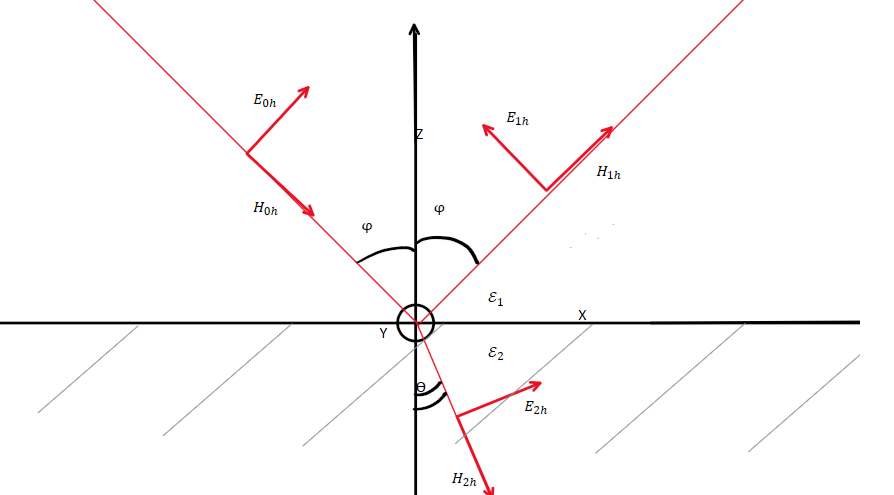
\includegraphics[width=0.5\textwidth]{Рис 7.PNG} % Вставка изображения. Укажите путь к вашему изображению вместо example-image
		\caption{Н поляризованная волна в среде с графеновым слоем} % Подпись к рисунку
		\label{fig:example7} % Метка для ссылки на рисунок
	\end{figure}
	
	Пусть на границу раздела 2х сред падает волна:
	
	\begin{equation}
		\begin{aligned}
			&\vec{E_{0H}} = \vec{y_0} E_{0H} e^{-ik_1(xcos(\phi) + zsin(\phi))} \\
			&\vec{H_{0H}} = -(\vec{x_0}sin(\phi) - \vec{z_0}cos(\phi)) \frac{E_{0H}}{Z_1}e^{-ik_1(xcos(\phi) + zsin(\phi))} \\ 
		\end{aligned}
	\end{equation}
	
	тогда отраженную и преломленную волну можно записать как:
	
	\begin{equation}
		\begin{aligned}
			&\vec{E_{1H}} = \vec{y_0}E_{1H} e^{-xcos(\phi) + zsin(\phi)} \\
			&\vec{H_{1H}} = -(\vec{x_0}sin(\phi) + \vec{z_0}cos(\phi)) \frac{E_{1H}}{Z_1} e^{-xcos(\phi) + zsin(\phi)} \\
			&\vec{E_{2H}} = \vec{y_0} E_{2H} e^{-ik_1(xcos(\theta) + zsin(\theta))} \\
			&\vec{H_{2H}} = -(\vec{x_0}sin(\theta) - \vec{z_0}cos(\theta)) \frac{E_{2H}}{Z_2}e^{-ik_1(xcos(\theta) + zsin(\theta))} \\ 
		\end{aligned}
	\end{equation}
	
	Так как граничные условия для $E$ выполняются ($[E_\tau] = 0$), то выполняются законы Снелиуса об углах падения и отражения.
	
	Для тангенсальной компоненты E можно записать 
	
	\begin{equation}
		E_{0H}e^{-ik_1zsin(\phi)} + E_{1H}e^{-ik_1zsin(\phi)} = E_{2H}e^{-ik_2zsin(\theta)}
	\end{equation}
	
	которое преабразуется в 
	
	\begin{equation*}
		\tag{79.1}
		E_{0H} + E_{1H} = E_{2H} 
	\end{equation*}
	
	Для $H$ граничные условия выглядят как $H_{\tau1} - H_{\tau2} = \delta E_{\tau2}$ или:
	
	\begin{equation}
		\frac{E_{0H}}{Z_1}cos(\phi) - \frac{E_{1H}}{Z_1}cos(\phi) - \frac{E_{2H}}{Z_2} = \delta E_{2H}
	\end{equation}
	
	Введем коефициент отражения и преломления:
	
	\begin{equation}
		\begin{aligned}
			R_H = \frac{E_{1H}}{E_{0H}} \\
			T_H = \frac{E_{2H}}{E_{0H}}
		\end{aligned}
	\end{equation}
	
	тогда получис систему:

	\begin{equation}
		\begin{cases}
			1 + R_H = T_H \\
			1 - R_H = \frac{Z_1 cos(\theta)}{cos(\phi)} (\delta + \frac{1}{Z_2})T_H \\
		\end{cases}
	\end{equation}
	
	Решая данную систему получим:
	
	\begin{equation}
		\begin{aligned}
			T_H = \frac{2 cos(\phi) Z_2}{cos(\phi)Z_2 + Z_1 cos(\theta) (1 + Z_2 \delta)} \\
			R_H = \frac{cos(\phi)Z_2 - Z_1cos(\theta)(Z_2 \delta+ 1)}{cos(\phi) Z_2 + Z_1 cos(\theta) (1 + Z_2 \delta)} 
		\end{aligned}
	\end{equation}
	
	
	\subsection{E поляризованная волна}
	
	\begin{figure}[h] % [h] означает, что рисунок будет размещен здесь, а не автоматически в конце раздела или страницы
		\centering % Выравнивание по центру
		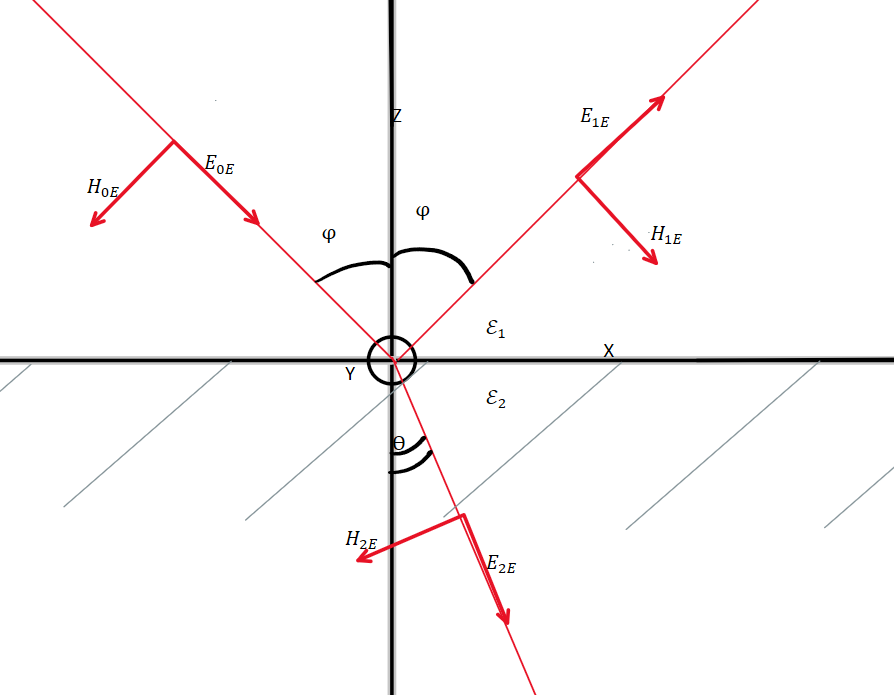
\includegraphics[width=0.5\textwidth]{Рис 8.PNG} % Вставка изображения. Укажите путь к вашему изображению вместо example-image
		\caption{E поляризованная волна в среде с графеновым слоем} % Подпись к рисунку
		\label{fig:example8} % Метка для ссылки на рисунок
	\end{figure}
	
	В этом случае граничные условия можно записать в виде:
	
	\begin{equation}
		\begin{cases}
			E_{0E} cos(\phi) - E_{1E} cos(\phi) = E_{2E} cos(\theta) \\
			\frac{E_{0E}}{Z_1} + \frac{E_{1E}}{Z_1} = \frac{E_{2H}}{Z_2} + \delta E_{2E} cos(\theta)
		\end{cases}
	\end{equation} 
	
	Вводя коефициент отражения и преломления:
	
	\begin{equation}
		\begin{aligned}
			R_E = \frac{E_{1E}}{E_{0E}} \\
			T_E = \frac{E_{2E}}{E_{0E}}
		\end{aligned}
	\end{equation}
	
	Тогда систему 84 можно переписать в виде:
	
	\begin{equation}
		\begin{cases}
			1 - R_E = T_E \frac{cos(\theta)}{cos(\phi)} \\
			1 + R_E = T_E (\frac{1}{Z_2} + \delta cos(\theta))Z_1
		\end{cases}
	\end{equation}
	
	Решением данной системы является:
	
	\begin{equation}
		\begin{aligned}
			T_E = \frac{2 cos(\phi ) Z_2}{cos(\theta) Z_2 + cos(\phi) Z_1 (1 + Z_2 \delta cos(\theta)} \\
			R_E = \frac{cos(\phi) Z_1 (1 + Z_2 \delta cos(\theta)) - cos(\theta) Z_2}{cos(\theta) Z_2 + cos(\phi) Z_1 (1 + Z_2 \delta cos(\theta))}
		\end{aligned}
	\end{equation} 
	
	\subsection{Волна падающая по нормали к поверхности} 
	
	H-поляризованная волна:
	
	\begin{equation}
		\begin{aligned}
				T_H = \frac{2  Z_2}{Z_2 + Z_1(1 + Z_2 \delta)} \\
			R_H = \frac{Z_2 - Z_1(Z_2 \delta + 1)}{ Z_2 + Z_1 (1 + Z_2 \delta)} 
		\end{aligned}
	\end{equation}
	
	E-поляризованная волна:
	
	\begin{equation}
		\begin{aligned}
			T_E = \frac{2 Z_2}{Z_2 +  Z_1 (1 + z_2 \delta) } \\
			R_E = \frac{ Z_1 (1 + Z_2 \delta) - Z_2}{ Z_2 +  Z_1 (1 + Z_2 \delta )}
		\end{aligned}
	\end{equation}
	
	
	\section{Выводы}
	
	В данной курсовой работе с помощью векторных потенциалов было полученно описание поля, порожденного электрическим диполем в плоскослоистой среде с графеновым слоем. Так же были выведены коефициенты отражения и преломления плоской электромагнитной волны в этой среде.
	
	\newpage 
	
	\section{Литература}
	
	\begin{itemize}
		\item [1] Тихонов А. Н. Самарский А. А. Уравнения математической физики: Учебное пособие - 6е издание Изд-во МГУ 1999. ISBN 5-211-04138-0 
		
		\item [2] Дмитриев В. И. Захаров Е. В. Метод интегральных уравнений в вычислительной электродинамике. МАКС Пресс 2008 - 316с ISBN 978-5-317-02657-8
		
		\item 3 Давыдов В. М. Теория низкочастотных электромагнитных полей в средах с тонкими анизотропными слоями и ее геофизические приложения. Новосибирск 1971.
		
		\item 4 S. A. Mikhailov
		Non-linear electromagnetic response of graphene
		Institute for Theoretical Physics II, University of Augsburg, D-86135
		Augsburg, Germany (Dated: February 5, 2008)
		
		\item 5 Linear and Nonlinear Optical Properties of Graphene: A Review
		Vipin Kumar Journal of Electronic Materials (2021) 50:3773–3799
		
		\item 6 Линейные и нелинейно-оптические свойства графена: обзор
		Випин Кумар - Журнал электронных материалов, 2021 - Springer
		
		\item 7 S. A. Mikhailov
		Institute for Theoretical Physics II, University of Augsburg, D-86135 Augsburg, Germany
		(Dated: October 22, 2018)
		
		\item 8 A. K. Geim and K. S. Novoselov, Nature Materials 6, 183 (2007).
		
		\item 9 Электромагнитное поле диполя в анизотропной среде
		© А.О. Савченко,1 О.Я. Савченко Журнал технической физики, 2005, том 75, вып. 1
		
		\item  10 Dmitriev V. I., Silkin A. N., Farzan R. Tensor green function for the system of maxwell’s equations in a layered medium // Computational Mathematics and Modeling. — 2002. — Vol. 13, no. 2. — P. 107–118. 
		
		\item 11 Вестник СибГУТИ. 2016. № 2
		УДК 621.396.67
		Тензорные функции Грина
		для расчета электромагнитных полей 
		от слоистых сферических структур
		Б. А. Панченко, Д. В. Денисов, А. М. Муcин, И. О. Скумотенко
	\end{itemize}
	
	
	
\end{document}